The \gls{object_handler_class} class is the interface to instances of a specific type. This class handles everything related to creating, retrieving, updating and deleting objects. It can be constructed through a method of the \gls{library_class}.

The \gls{object_handler_class} provides two forms of access to the underlying database: direct and managed. When using direct access, you are responsible for allocating objects. Whether you do that on the stack or the heap is up to you. When using managed access, objects are allocated on the heap by the \gls{object_handler_class}. Additionally, they can be cached in memory (automatically or manually) to reduce disk access.

\subsection{Construction}
%TODO: Creating an ObjectHandler. 
% What about multiple ObjectHandlers?
% Member and MemberList.

\subsection{Direct Access}

There are two ways in which you can create new instances. The first is by using the \code{create} method. This method will add a new row to the \gls{instance_table} with all default values. It also takes a pointer parameter. If not null, the instance is immediately retrieved. See Listing~\ref{lst:object_handler:instance_create_direct}.

\lstinputlisting[caption={Creating a new instance.}, label={lst:object_handler:instance_create_direct}]{snippets/instance_create_direct.cpp}

The second way is with the \code{insert} method. This method takes a reference to an object that will be added to the database with all its values. Just as with the \code{create} method, the object that you pass should not have a valid identifier yet. After insertion, the identifier will be set. See Listing~\ref{lst:object_handler:instance_insert_direct}.

\lstinputlisting[caption={Inserting a new instance.}, label={lst:object_handler:instance_insert_direct}]{snippets/instance_insert_direct.cpp}

After modifying an object, you can update the database by passing the object to the \code{update} method. See Listing~\ref{lst:object_handler:instance_update_direct}.

\lstinputlisting[caption={Updating an existing instance.}, label={lst:object_handler:instance_update_direct}]{snippets/instance_update_direct.cpp}

Instances can be retrieved by their identifier. The \code{get} method takes an identifier parameter and a reference to the object to which all values are written. Just as with the \code{create} method, the identifier should not have been set yet and is initialized after retrieval. See Listing~\ref{lst:object_handler:instance_get_direct}.

\lstinputlisting[caption={Retrieving an instance.}, label={lst:object_handler:instance_get_direct}]{snippets/instance_get_direct.cpp}

Deleting an instance from the database is simple. Just call the \code{del} method with the instance identifier. See Listing~\ref{lst:object_handler:instance_delete_direct}.

\lstinputlisting[caption={Deleting an instance.}, label={lst:object_handler:instance_delete_direct}]{snippets/instance_delete_direct.cpp}

\subsection{Managed Access}

There is a managed equivalent to all \code{create}, \code{insert}, \code{update} and \code{get} methods. They use \code{shared\_ptr}s instead of references. Pointers to the allocated objects can be stored in a cache such that repeated retrieval does not require any disk access.

The first time an instance is created, accessed, inserted, etc., a new entry is added to the cache. Depending on the default caching method, either an owning pointer (\code{shared\_ptr}), non-owning pointer (\code{weak\_ptr}), or no pointer is stored. When you try go get an instance for which an entry exists in the cache, the following will happen depending on what the entry holds:

\begin{itemize}
	\item \textbf{Strong}: the \code{shared\_ptr} is returned directly.
	\item \textbf{Weak}: the \code{weak\_ptr} is \code{lock}'ed. If there still is an owning pointer around, a new owning pointer is constructed and returned. Otherwise, the database is queried for the object.
	\item \textbf{None}: The database is queried for the object.
\end{itemize}

The default caching method is \code{alex::CacheMethod::Weak}. If you for example retrieve an object and keep around the pointer, another retrieval will construct another \code{shared\_ptr} pointing to the same object from the \code{weak\_ptr} that is stored in the cache. No disk access would be needed until all owning pointers are discarded. To change how objects are cached by default, use the \code{setDefaultCacheMethod} method.

It is also possible to manually control the way each instance is cached using the \code{setCacheMethod} and \code{clearCache} methods. Additionally, cache entries can be modified in bulk using the various \code{release*} and \code{clear} methods. Finally, you can retrieve and inspect the entire cache with the \code{getCache} method.

\begin{figure}[H]
	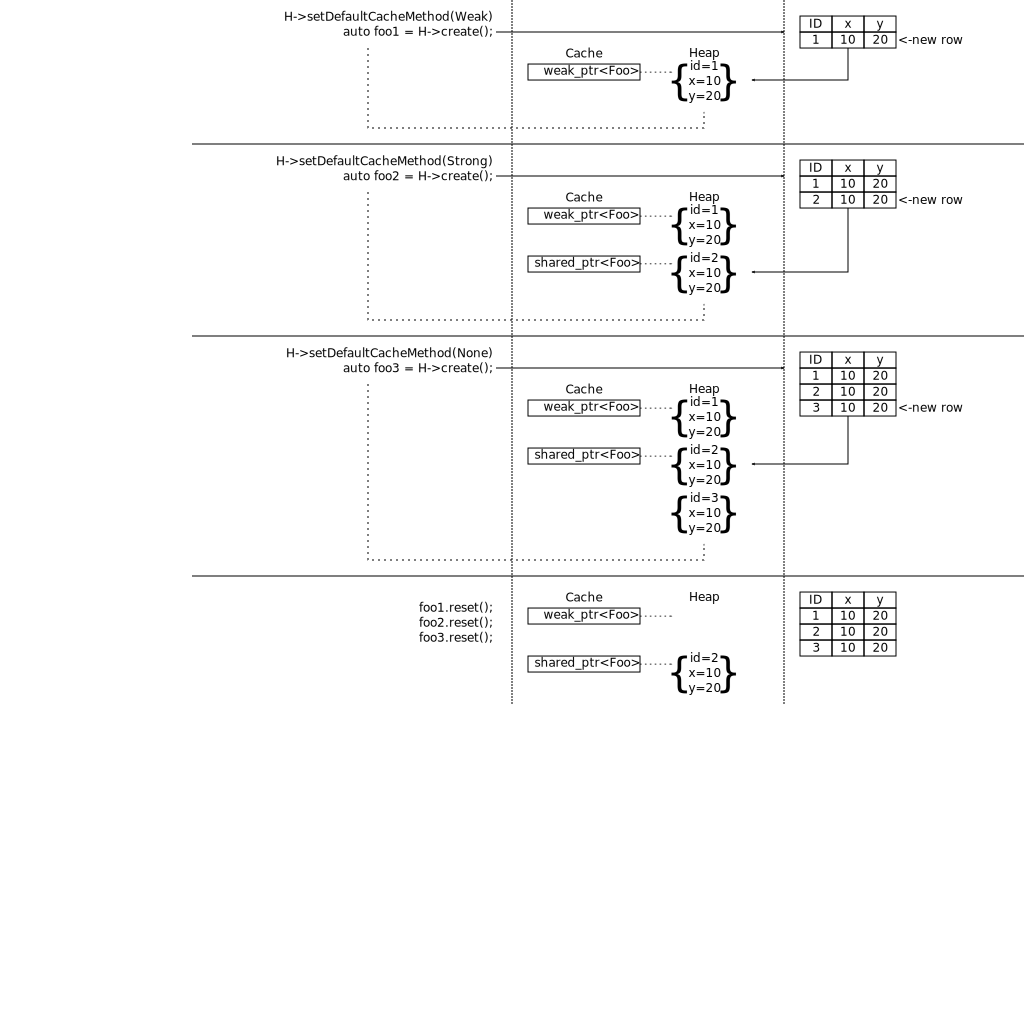
\includegraphics[width=1\textwidth]{figures/create.pdf}
	\caption{Creating new instances.}\label{fig:object_handler:create}
\end{figure}

\begin{figure}[H]
	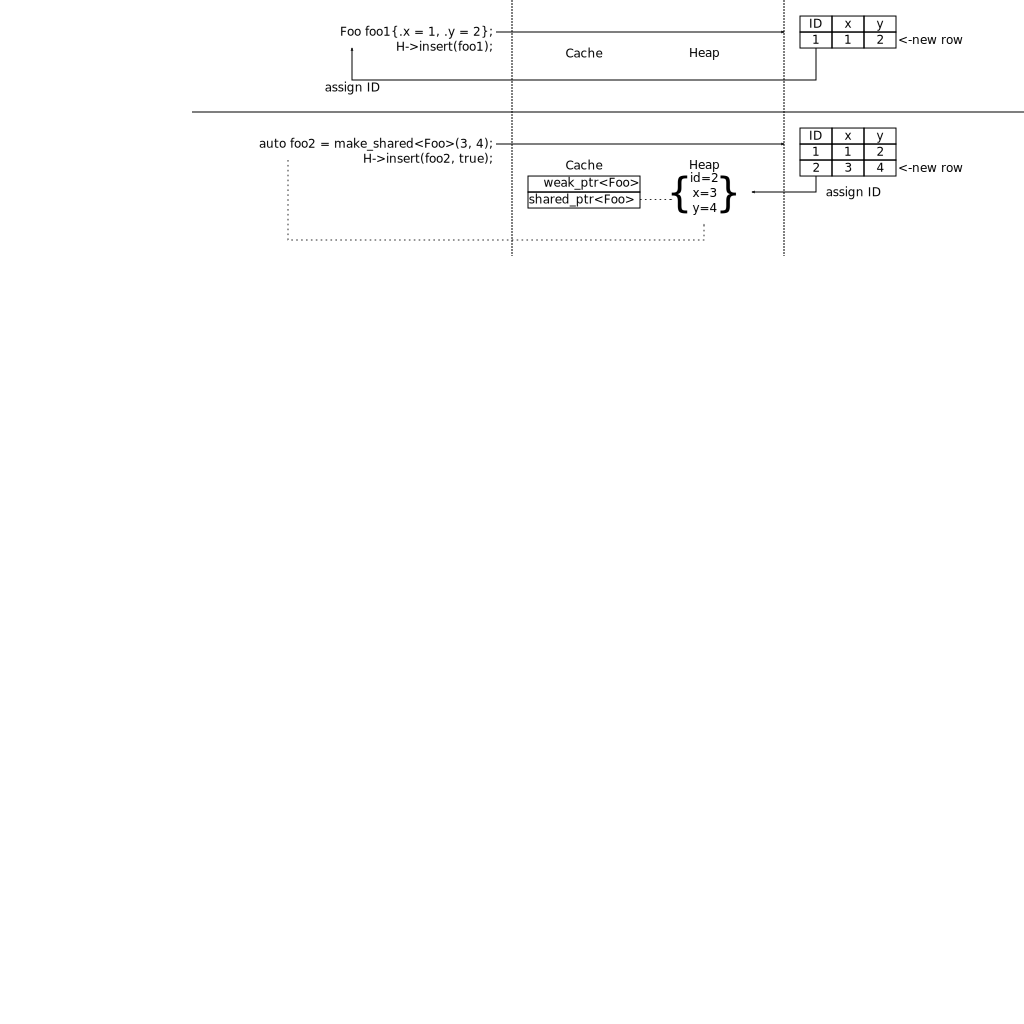
\includegraphics[width=1\textwidth]{figures/insert.pdf}
	\caption{Insert existing objects.}\label{fig:object_handler:insert}
\end{figure}

\subsection{...}

% TODO: Explain how references between objects can be kept valid.